\section{Introduction}
%\paragraph{Problem statement}
%    \subparagraph{language evolution}
    A human language is comprised of a pronunciation system and a writing system, both evolving and changing over time. An important part of historical phonology is about reconstructing the historical pronunciation system and its pattern of evolution, sometimes as drastic as the three examples in Table \ref{tab: Evolution example}\footnote{Pronunciations in this paper are all transcribed with International Phonetic Alphabet (IPA). See \href{https://www.internationalphoneticalphabet.org/ipa-sounds/ipa-chart-with-sounds/}{https://www.internationalphoneticalphabet.org/ipa-sounds/ipa-chart-with-sounds/} for IPA characters and sounds.}. 
    \begin{table}[ht]
    \centering
    \small
    \resizebox{\linewidth}{!}{
        \begin{tabular}{ccccccc}
        \hline
        \textbf{Char} & \textbf{T} & \textbf{L} & \textbf{S} & \textbf{Y} & \textbf{Q} & \textbf{M} \\
        \hline
        \begin{CJK*}{UTF8}{gbsn}顺\end{CJK*} & \textipa{[\textdctzlig iuin]} & \textipa{[\textctz iu@n]} & \textipa{[Ciu@n]} & \textipa{[Cy@n]} & \textipa{[\textrtails un]} & \textipa{[\textrtails u@n]}\\
        \begin{CJK*}{UTF8}{gbsn}席\end{CJK*} & \textipa{[zi\textturna k]} & \textipa{[zi@k]} & \textipa{[sit]} & \textipa{[si]} & \textipa{[si]} & \textipa{[\textctc i]}\\
        \begin{CJK*}{UTF8}{gbsn}乏\end{CJK*} & \textipa{[biu\textturna p]} & \textipa{[viu\ae p]} & \textipa{[fap]} & \textipa{[fau]} & \textipa{[fa]} & \textipa{[fa]}\\
        \hline				
        \end{tabular}}
    \caption{Reconstructed pronunciations (in IPA) of three characters over 6 Chinese historical periods: MiddleTang - T, LateTang - L, Song - S, Yuan - Y, MingQing - Q and Modern - M. See \figref{fig:timeline} for corresponding timeline.}
    \label{tab: Evolution example}
    \end{table}
    Studies on Chinese historical phonology using modern comparative methods began in 1915 ~\cite{karlgren_etudes_1915}, followed by various attempts to reconstruct MiddleTang Chinese~\cite{TheReconstructionofAncientChinese,Pulleyblank_1991,wang_l_hanyu_2012}.
    % \KZ{Just say an important part of Phonology is about predicting or reconstructing the historical pronunciation. This is important not only for academic interests, but also useful in preserving very rare languages.} 
    % \MY{These two sentences are not linked, we should still say 1 sentence that there's some study working on language evolution and phonological reconstruction, with a few citations.}
    These studies reveal the causes and trends of language evolution and contribute to the study of ancient literature resources.
    % \MY{are you referring to glyphs? they are linguistic traces too.}
    %\subparagraph{difficulties for reconstructing ancient Chinese}
     
     Historical scripts are often preserved in tangible forms, yet the transmission of pronunciation through successive generations is more susceptible to variation and distortion. Across linguistic domains, the systematic evolution of phonetics frequently eludes precise documentation. In the realm of Sinological phonology inquiry, the logographic nature of Chinese script primarily conveys semantic content, offering limited insight into phonetic attributes (See Figure \ref{fig:different_pronunciation}).
     % \MY{I rewrite these sentences, please make sure to say that Chinese characters are logographic, meaning they represent words or morphemes rather than sounds directly.: Historical scripts are often preserved in tangible forms, yet the transmission of pronunciation through successive generations is susceptible to variation and distortion. Across linguistic domains, the systematic evolution of phonetics frequently eludes precise documentation. In the realm of Sinological phonological inquiry, the ideographic nature of Chinese script primarily conveys semantic content, offering limited insight into phonetic attributes.} 
      Therefore, unlike phonograms in many other common languages, Chinese writing is considered logographic, meaning each phoneme or syllable does not correspond to a specific character.
    \begin{figure}[ht]
        \centering
        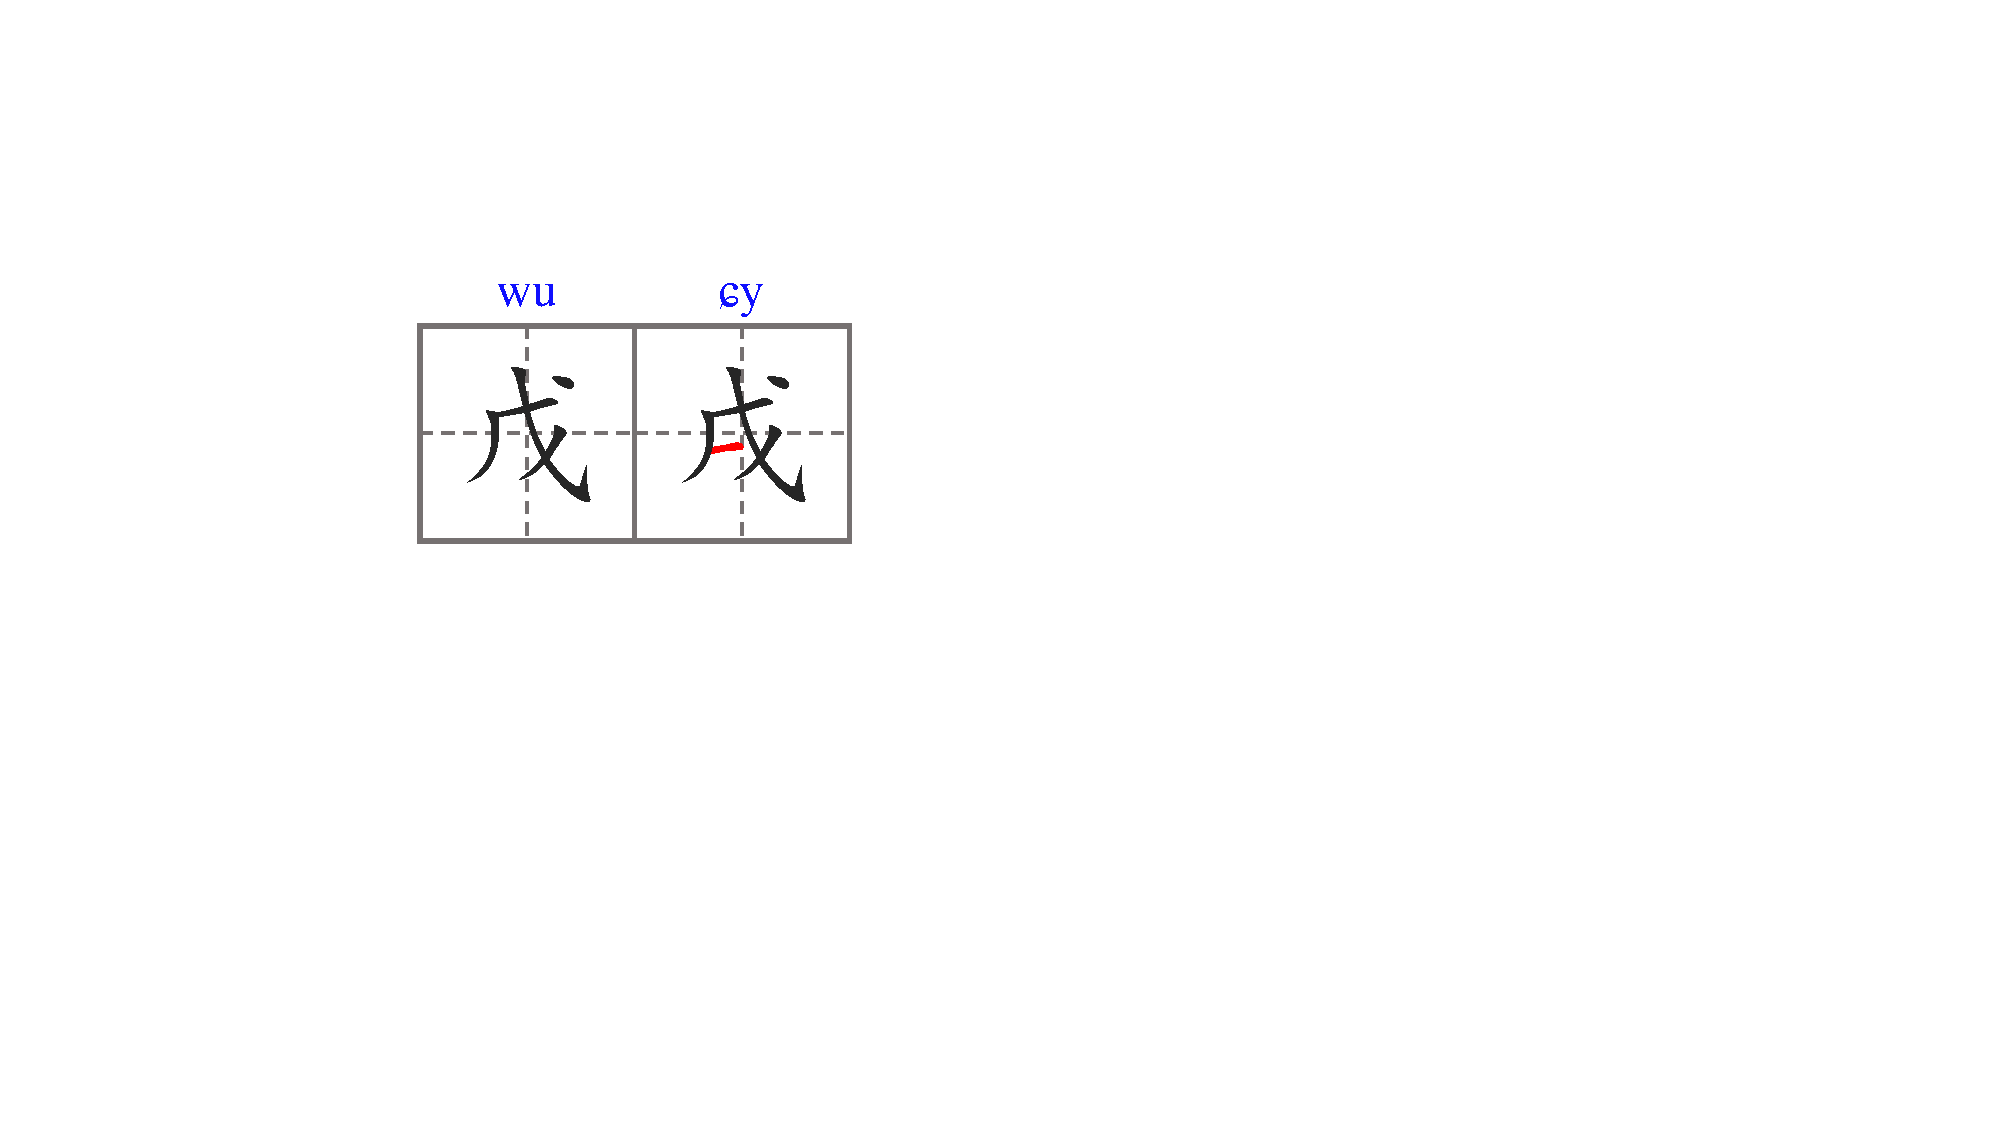
\includegraphics[width=2cm]{images/diff_pro.pdf}
        \caption{Similar characters with different pronunciation, showing that Chinese characters are not indicative of
        sound.} \label{fig:different_pronunciation}
    \end{figure}
     
%\paragraph{existing problems}
%    \subparagraph{how linguists reconstruct}
    When attempting to reconstruct the Chinese phonological system for a certain historical period, only limited resources of pronunciation records are provided. Current studies are based on a rhyming dictionary \textit{Guangyun} \cite{guangyun_1936} published in AD 601. From then on, Chinese linguists in different dynasties inherited the taxonomy of character pronunciations in \textit{Guangyun}, and used the comparative method to group similar-sounding characters into the same category. Combined with xeno-Chinese transliteration\footnote{Translation materials between Chinese and foreign languages in a specific period, e.g. Translation of Sutras published in MiddleTang can correspond Sanskrit (phonographic language) to MiddleTang Chinese (logographic language).}
    % \XJ{What is xeno-Chinese transcription?}
    , modern dialect pronunciation, etc., the Chinese pronunciation system can be partially reconstructed ~\cite{zhao_hanyu_2015}. 

%    \subparagraph{current problem of reconstruction}
    % \KZ{Why therefore?} 
    Given ample attempts and combining different linguistic discoveries, the rule-based reconstruction method has its inherent limitations. 
    % \MY{I rephrase this first sentence please check: Given ample attempts and combining different linguistic discoveries, rule-based reconstruction method has its inherent limitations. }
    % \KZ{The following three points need to be rephrase. I can't grasp what you are talking about after reading it.} 
    First, the pronunciation is reconstructed within each category but not for each character, making the result neither intuitive nor easy to search.
    Second, current reconstruction results cannot cover all Chinese characters' pronunciation over all historical periods. Chinese language system's evolution is not strictly under the taxonomy of \textit{Guangyun} (See Sec. \ref{sec:dataset}), making it impossible to always apply rule-based change patterns on a whole category\footnote{For the reconstruction of the intermediate dynasties (Yuan, Ming and Qing dynasties), the linguistic reconstruction we use can only cover some of the Chinese characters for which rhyming patterns can be hypothesized based on the available documentary materials.}. 
    Third, current results are not fully digitized but only in printed versions. 
    As a matter of fact, the process of character-wise pronunciation reconstruction is complex, encompassing the entirety of Chinese characters across various historical eras, and necessitates prior knowledge in linguistics, thereby calling for further refinement. 
    % \MY{As a matter of fact, the process of character reconstruction is complex, encompassing the entirety of Chinese characters across various historical eras, and necessitates a foundation in linguistics, thereby calling for further refinement.}
    
    Recently, several computer-assisted methods have been proposed to reconstruct ancient Chinese pronunciation, including~\citet{chang_wikihan_2022}'s comparative Chinese dialect dataset and~\citet{kim_transformed_2023}'s approach of applying transformer model on this dataset to rebuild ancient Chinese pronunciation. However, the reconstruction results are limited to a specific historical period, i.e., MiddleTang Chinese pronunciation. Hence, we attempt to build a time-aware dataset and use a temporal factor-embedded model to complete the reconstruction at an arbitrary time point.  
    % \MY{Here you should use 1-2 sentences to say what you've done and how this paper differs from these existing computer-assisted ones.}
    % \KZ{middle chinese?}

%    \paragraph{our work \& contribution}
The contribution of this paper is as follows:
\begin{itemize}
\item We build a chronological ACP (\textbf{A}ncient \textbf{C}hinese \textbf{P}ronunciation) dataset by combining and digitizing the \textit{Guangyun}-based Chinese character taxonomy and the existing ancient Chinese reconstruction results in linguistics, offering 70,943 pronunciation entries for 17,001 Chinese characters (\secref{sec:dataset}). 
\item Aiming to interpolate and extrapolate the reconstruction result to any time point, we propose a transformer-based pronunciation reconstruction model (\secref{sec:model}), . With additional language features encoded, our model achieves the best accuracy score on random-split, phonetic distinction, and reduced training data evaluations compared to baseline models (\secref{sec:evaluations}), showing its ability to refine incomplete phonological reconstruction results of traditional linguistics. 
% \XJ{did not see \textit{ordinary}, \textit{hard} and \textit{low input-resource} reconstruction tasks in experiment part.}
\item By using a chronological dataset, our time-aware model also has the ability to reconstruct the pronunciation for a given period when the information for training is sparse or even completely missing in the current ACP dataset. 
\end{itemize}
% Fortunately, Modern studies in Chinese linguistics have provided some preliminary reconstruction results of ancient Chinese pronunciation. A relatively comprehensive result can be found in \textit{History of Chinese Phonetics} where the exact IPA
% % q: IPA(wiki?)
% form of pronunciation is attached to each category under the taxonomy of \textit{Qieyun}, a classification system of Chinese characters that originated in 601 D.C.. The reconstruction is conducted over various dynasties including MiddleTang(581-836), LateTang(836-960), Song(960-1279), Yuan(1279-1368), MingQing(1368-1911) and modern Chinese(Mandarin). We improve this reconstruction result under the following three aspects:  \KZ{You wanna give some examples of Qie Yun here. Maybe a small pic?} Thirdly, the results are not fully digitized but only has printed version.
% For computer assisted ancient Chinese reconstruction task, our work has the following contributions: \KZ{These don't sound like contributions. Where are the adjectives and superlatives?}


